\documentclass[11pt, a4paper]{article}
\usepackage{polski}
\usepackage[utf8]{inputenc}
\usepackage[T1]{fontenc}
\usepackage[export]{adjustbox}
\usepackage{graphicx}
\usepackage{amsmath} 
\usepackage{listings}
\usepackage{color}
\usepackage{marvosym}
\usepackage{geometry}
\usepackage{float}
\usepackage{booktabs}
\usepackage{multirow}
\usepackage{titlesec}
\usepackage{hyperref}
\usepackage{tabularx}

\geometry{margin=1.2in}
\usepackage[final]{pdfpages}

\newcommand{\fbi}{\leavevmode{\parindent=1em\indent}}

\definecolor{dkgreen}{rgb}{0,0.6,0}
\definecolor{gray}{rgb}{0.5,0.5,0.5}
\definecolor{mauve}{rgb}{0.58,0,0.82}

\lstset{
	frame=tblr,
	language=R,
	aboveskip=3mm,
	belowskip=3mm,
	showstringspaces=false,
	columns=flexible,
	basicstyle={\small\ttfamily},
	numbers=left,
	numberstyle=\tiny\color{gray},
	keywordstyle=\color{blue},
	commentstyle=\color{dkgreen},
	stringstyle=\color{mauve},
	breaklines=true,
	mathescape=false,
	breakatwhitespace=true,
	tabsize=3,
	inputencoding=utf8,
	extendedchars=true,
	literate=
	{ą}{{\k{a}}}1
	{Ą}{{\k{A}}}1
	{ę}{{\k{e}}}1
	{Ę}{{\k{E}}}1
	{ó}{{\'o}}1
	{Ó}{{\'O}}1
	{ś}{{\'s}}1
	{Ś}{{\'S}}1
	{ł}{{\l{}}}1
	{Ł}{{\L{}}}1
	{ż}{{\.z}}1
	{Ż}{{\.Z}}1
	{ź}{{\'z}}1
	{Ź}{{\'Z}}1
	{ć}{{\'c}}1
	{Ć}{{\'C}}1
	{ń}{{\'n}}1
	{Ń}{{\'N}}1
}

\renewcommand\lstlistingname{Listing}

\titleclass{\subsubsubsection}{straight}[\subsection]
\newcounter{subsubsubsection}[subsubsection]
\renewcommand\thesubsubsubsection{\thesubsubsection.\arabic{subsubsubsection}}
\renewcommand\theparagraph{\thesubsubsubsection.\arabic{paragraph}}

\titleformat{\subsubsubsection}
  {\normalfont\normalsize\bfseries}{\thesubsubsubsection}{1em}{}
\titlespacing*{\subsubsubsection}
{0pt}{3.25ex plus 1ex minus .2ex}{1.5ex plus .2ex}

\makeatletter
\renewcommand\paragraph{\@startsection{paragraph}{5}{\z@}
  {3.25ex \@plus1ex \@minus.2ex}
  {-0em}
  {\normalfont\normalsize\bfseries}}
\renewcommand\subparagraph{\@startsection{subparagraph}{6}{\parindent}
  {3.25ex \@plus1ex \@minus .2ex}
  {-1em}
  {\normalfont\normalsize\bfseries}}
\def\toclevel@subsubsubsection{4}
\def\toclevel@paragraph{5}
\def\toclevel@paragraph{6}
\def\l@subsubsubsection{\@dottedtocline{4}{7em}{4em}}
\def\l@paragraph{\@dottedtocline{5}{10em}{5em}}
\def\l@subparagraph{\@dottedtocline{6}{14em}{6em}}
\makeatother

\setcounter{secnumdepth}{4}
\setcounter{tocdepth}{4}

\hypersetup{pageanchor=false}

\setlength\parindent{3pt}

\renewcommand{\labelenumi}{\alph{enumi}.} 

\date{\today}

\begin{document}

\begin{titlepage}

\newcommand{\HRule}{\rule{\linewidth}{0.5mm}} 
\center 

\textsc{\LARGE Politechnika Wrocławska}\\[1.5cm] 
\textsc{\Large Inteligencja Obliczeniowa i jej zastosowania}\\[0.5cm] 
\HRule \\[0.5cm]
{ \huge \bfseries Badanie algorytmu genetycznego z zakresu optymalizacji globalnej dla wybranej funkcji testowej. Przeprowadzenie pomiarów dla algorytmu hybrydowego i optymalizacji rojem cząstek }\\[0.5cm] 
\HRule \\[1.6cm]
 
\begin{minipage}{0.4\textwidth}
\begin{flushleft} \large
\emph{Autorzy:}\\
Paweł  \textsc{Andziul} 200648 \\
Marcin  \textsc{Słowiński} 200638 \\
\end{flushleft}
\end{minipage}
~
\begin{minipage}{0.4\textwidth}
\begin{flushright} \large
\emph{Prowadzący:} \\
dr hab. inż. Olgierd \textsc{Unold}, prof. nadzw. PWr
\end{flushright}
\end{minipage}\\[4cm]

\vfill 
{\large 26 kwietnia 2017}\\[3cm] 

\end{titlepage}

\tableofcontents

\newpage
\section{Wprowadzenie}
\paragraph{}
[todo]
Algorytm genetyczny – algorytm heurystyczny, który swoim działaniem przypomina działanie ewolucji w~naturze. Osobniki będące zbyt słabe zostają wyeliminowane z~populacji w~kolejnych pokoleniach, a~na ich miejsce przyjmowane są lepsze, silniejsze, bardziej podatne adaptacji. Algorytmy te zakładają możliwość mutacji i~krzyżowania wśród potomków, przez co nie zawsze są oni silniejsi od poprzednio wyeliminowanych członków. Dodatkowo wprowadzają pojęcie elity, która jest bezpośrednio przenoszona do następnego - teoretycznie lepszego pokolenia.



\textit{dla wybranej funkcji własnej funkcje krzyżowania (dla branina)
dla tsp (np--trudny) genetyczny -- tsplib wykorzystać do badań (2--3 instancje srednie male duze) z wlasnym operatorem z domyslnym
algorytm ga z lokalnym wyszukiwaniem, dla komiwojażera, założyć czy ma lepsze wartości, czy szybciej zbiega, jak operatory się zachowują,
psoptim, dla jednej funkcji i komiwojażera}



\fbi
W ramach laboratorium należało przeprowadzić testy algorytmu genetycznego dla różnych parametrów. Jako benchmark oceny należało użyć pakietu ,,getGlobalOpts'' oraz języka R.

\fbi
Pomiary wykonywano na 2 różnych jednostkach roboczych. Ich parametry nie są istotne z~punktu widzenia analizy i~możliwości porównania rezultatów.



\section{Implementacja}
\paragraph{}
Poniżej zamieszczono kody skryptów w~języku R przygotowanych w~celu umożliwienia przeprowadzenia pomiarów.

\lstinputlisting[label=lst:skryptGlowny,caption=Skrypt w~języku R wykorzystany do badań optymalizacji funkcji,firstline=1,lastline=500]{./assets/skrypt_lab35_funkcja.R}

\fbi
Skrypt przygotowano w~sposób który umożliwia w~pełni automatyczne przeprowadzenie wszystkich pomiarów. Jednocześnie wszystkie wykresy mogą być natychmiast podmienione w~sprawozdaniu. Poniżej pokrótce omówiono podstawowe parametry.


\begin{itemize}
	\item nOfRuns
	
	Ilość powtórzeń dla każdego pomiaru w~celu uśrednienia.
	
	\item colors, series
	
	Wektory kolorów i~nazw kolejnych serii pomiarowych. 
	
	\item params
	
	Macierz parametrów domyślnych algorytmu dla każdej z~serii. W każdym wierszu kolejno są zawarte: p. mutacji, p. krzyżowania, rozmiar populacji, ilość iteracji oraz kolor serii na wykresach.
	
	\item functions
	
	Wektor nazw funkcji dla których przeprowadzane są kolejno pomiary.
	
\end{itemize}

Całość informacji niezbędnych do przeprowadzenia obliczeń odczytywana jest na podstawie nazwy funkcji z~pakietu ,,globalOptTests''. Są to: rozmiar problemu (ilość parametrów), domyślne ograniczenia, wartość w~danym punkcie oraz optimum dla domyślnych ograniczeń.

\fbi
Dodatkowo warto wspomnieć, iż algorytm ,,psoptim'' w trochę inny sposób niż genetyczny przekazuje parametry do ewaluowanej funkcji. W tym przypadku jest to macierz w której kolumny to kolejne parametry natomiast wiersze odpowiadają kolejnym cząstkom. Zatem wymagane jest by funkcja umożliwiała wektorową ewaluację parametrów. Z~uwagi na wykorzystywanie funkcji z pakietu ,,globalOptTests'' wymagało to utworzenia odpowiedniego wrappera.


\fbi
Poniżej skrypt wykorzystany dla problemu komiwojażera.

\lstinputlisting[label=lst:skryptKomiwojazer,caption=Skrypt w~języku R wykorzystany do badań dla problemu komiwojażera,firstline=1,lastline=500]{./assets/skrypt_lab35_komiwojazer.R}


\subsection{Opis własnych operatorów}
\paragraph{}
Własna funkcja mutacji została utworzona w taki sposób by nie doprowadzić do sytuacji, w której przekroczona zostanie minimalna lub maksymalna wartość populacji. 

\fbi
Jej działanie opiera się na wybraniu minimalnej jednostki z populacji i podmianie innej, losowej na znaleziona minimalną. Gwarantuje to niepojawienie się z populacji wartości nieoczekiwanej, lecz tylko te otrzymane podczas działania algorytmu.


\newpage
\section{Przebieg badań dla problemu optymalizacji rzeczywistej Hartman6}
\paragraph{}
Badania przeprowadzono dla algorytmu genetycznego w wersji podstawowej, ze zmienioną funkcją mutacji oraz hybrydowej, a także dla optymalizacji rojem cząstek (PSO).

\fbi
Hartman6 jest funkcją określoną dla ilości parametrów równej 6. Na ilustracji (rys.~\ref{fig:hartman61}) przedstawiono jej wykres dla pierwszych dwóch. Poniżej zamieszczono jej wzór (\ref{eq:hartman6}).

\begin{equation}\label{eq:hartman6}
f(\boldsymbol{x}) = - \sum_{i=1}^{4} c_i \exp[- \sum_{j=1}^{6} a_{ij}(x_j - p_{ij})^2]
\end{equation}

, gdzie $ x_i \in [0, 1] $, $ i~\in \{1, ..., 6\} $.


\begin{figure}[H]
	\centering
	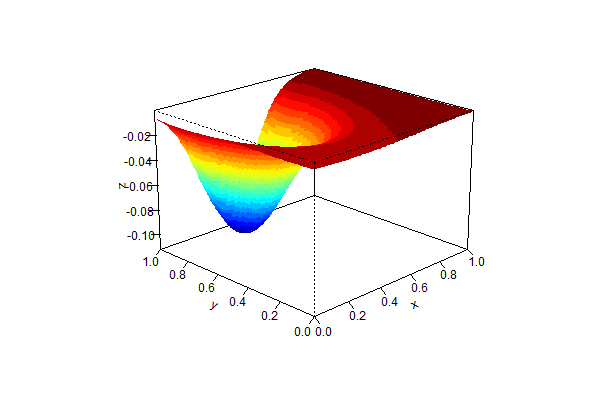
\includegraphics[width=0.95\textwidth]{./assets/Hartman6_overview.png}
	\caption{Wykres funkcji Hartman6}
	\label{fig:Hartman6_overview}
\end{figure}

\fbi
Na kolejnych stronach zamieszczono wyniki badań porównawczych mutacji przeprowadzonych na algorytmie.

\begin{figure}[H]
	\centering
	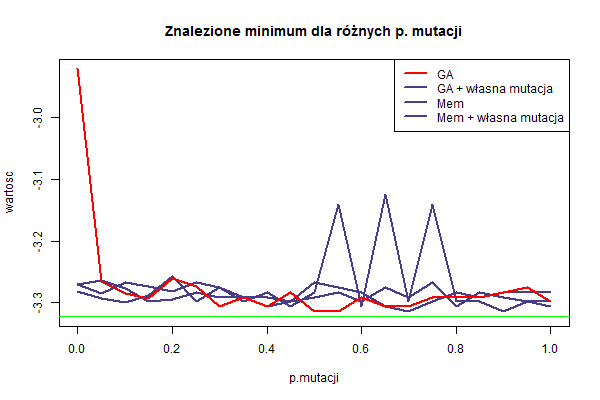
\includegraphics[width=0.95\textwidth]{./assets/Hartman6mut1.png}
	\caption{Wykres funkcji Hartman6}
	\label{fig:Hartman6mut1}
\end{figure}

\begin{figure}[H]
	\centering
	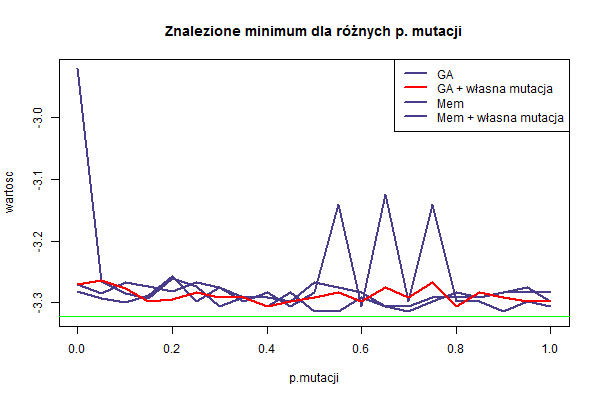
\includegraphics[width=0.95\textwidth]{./assets/Hartman6mut2.png}
	\caption{Wykres funkcji Hartman6}
	\label{fig:Hartman6mut2}
\end{figure}

\begin{figure}[H]
	\centering
	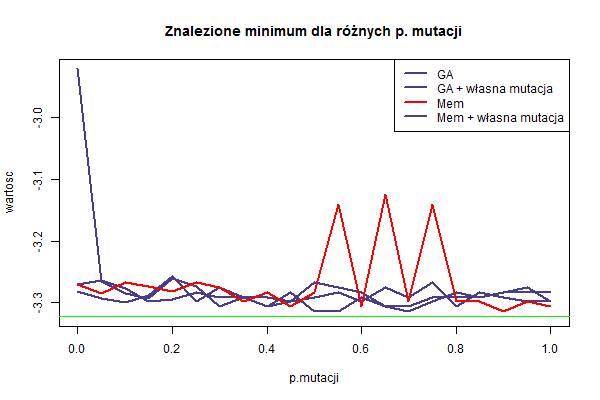
\includegraphics[width=0.95\textwidth]{./assets/Hartman6mut3.png}
	\caption{Wykres funkcji Hartman6}
	\label{fig:Hartman6mut3}
\end{figure}

\begin{figure}[H]
	\centering
	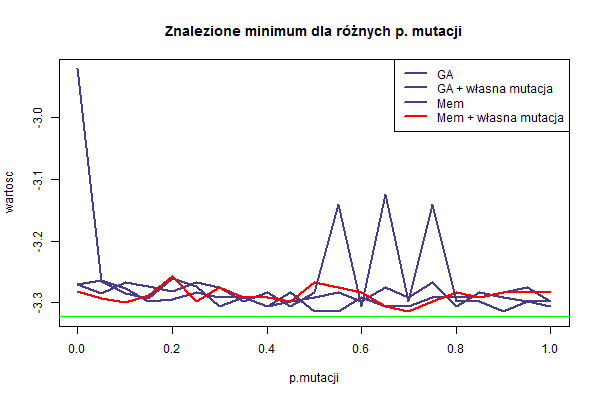
\includegraphics[width=0.95\textwidth]{./assets/Hartman6mut4.png}
	\caption{Wykres funkcji Hartman6}
	\label{fig:Hartman6mut4}
\end{figure}

\fbi
Z wykresów badań można odczytać zbliżone wyniki dla różnych funkcji mutacji.

\fbi
Żadna z funkcji nie osiągnęła minimum co świadczy o tym, że sama mutacja do tego nie wystarczy.

\fbi
Zauważalny jest również niski wpływ własnej funkcji mutacji na otrzymywane wyniki. Pod względem jakości rozwiązań nie odstaje ona od istniejących implementacji.

\fbi
Na wykresach można zauważyć znaczące pogorszenie się wyników dla funkcji memetycznej z domyślną funkcją mutacji. W przedziale 0.5-0.8 wygenerowała ona wyniki oddalone od średniej pozostałych.


\newpage
\section{Przebieg badań dla problemu komiwojażera}
\paragraph{}
Przeprowadzono badania z zakresu optymalizacji marszruty dla problemu komiwojażera. Wykorzystano trzy instancje problemu z biblioteki TSPLIB:

\begin{itemize}
	\item eil51
	\item eil76
	\item eil101
\end{itemize}

\fbi
Jakość rozwiązań wyraża się wzorem:

\begin{equation}\label{eq:tspquality}
quality\ of\ solution = \frac{shortest\ known \ path}{found\ path} * 100\%
\end{equation}

\fbi
Na ilustracji (rys.~\ref{fig:tsppop}) przedstawiono wyniki pomiarów dla różnych rozmiarów populacji.

\begin{figure}[H]
	\centering
	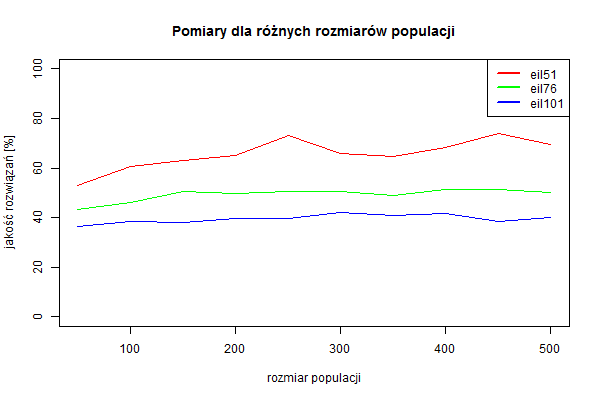
\includegraphics[width=0.95\textwidth]{./assets/tsp_pop.png}
	\caption{Jakość rozwiązań dla różnych rozmiarów populacji}
	\label{fig:tsppop}
\end{figure}

\fbi
Dla wszystkich badanych instancji zwiększenie populacji wpłynęło pozytywnie na jakość otrzymanego rozwiązania, co najbardziej obrazuje instancja "eli51", która poprawiła się o~ok. 20 punktów procentowych w badanym obszarze.


\fbi
Na ilustracji (rys.~\ref{fig:tspmut}) przedstawiono wyniki pomiarów dla różnych wartości p. mutacji.

\begin{figure}[H]
	\centering
	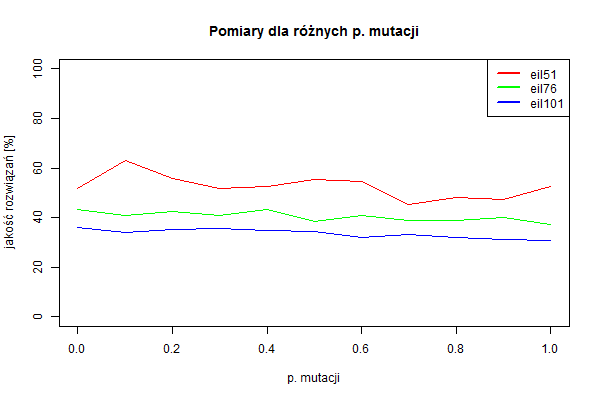
\includegraphics[width=0.95\textwidth]{./assets/tsp_mut.png}
	\caption{Jakość rozwiązań dla różnych wartości p. mutacji}
	\label{fig:tspmut}
\end{figure}

\fbi
Z powyższego wykresu nie można ustalić wpływu prawdopodobieństwa mutacji na jakość rozwiązań dla instancji "eli76" i "eli101". Dla instancji "eli51" jakość niestabilnie spada wraz ze wzrostem prawdopodobieństwa mutacji.


\fbi
Na ilustracji (rys.~\ref{fig:tspmutcust}) przedstawiono wyniki pomiarów dla różnych wartości p. mutacji z~niestandardowym operatorem.

\begin{figure}[H]
	\centering
	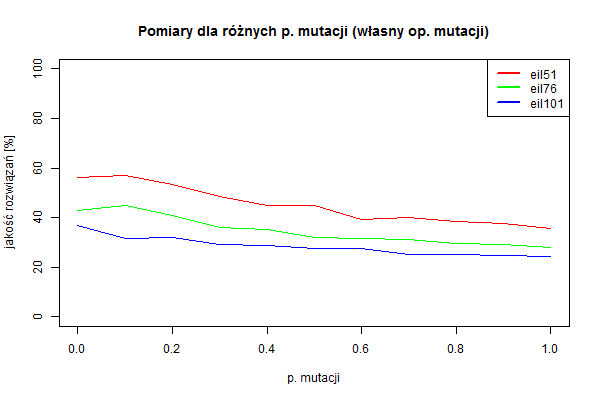
\includegraphics[width=0.95\textwidth]{./assets/tsp_mut_custom.png}
	\caption{Jakość rozwiązań dla różnych wartości p. mutacji (dla własnego operatora)}
	\label{fig:tspmutcust}
\end{figure}

\fbi
W przypadku własnej funkcji mutacji jakość rozwiązań problemu komiwojażera widocznie pogarsza u wszystkich instancji wraz ze wzrostem prawdopodobieństwa mutacji. W~przypadku "eli51" jest to nawet 20 punktów procentowych.


\newpage
\section{Badania algorytmów dla różnych wartości ich unikalnych parametrów}
\paragraph{}
Algorytmy memetyczny i PSO posiadają własne wartości unikalne, których zmiana może wpłynąć na otrzymywane wyniki. Poniżej przedstawiono wykresy przedstawiające otrzymane wartości dla zmieniających się wybranych parametrów.

\fbi
Badania przeprowadzono w przedziale 0-1 z krokiem co 0,01. Otrzymane wyniki są uśrednionymi z 15 iteracji.

\begin{figure}[H]
	\centering
	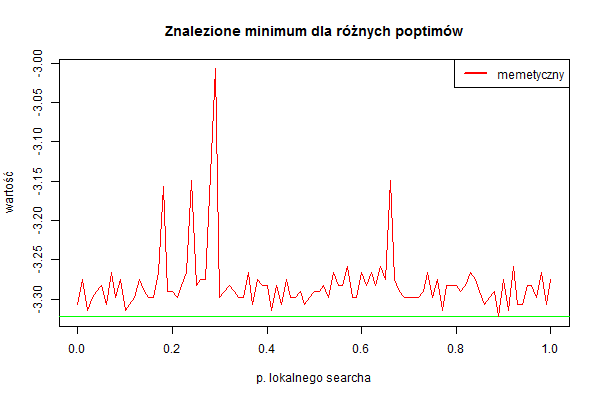
\includegraphics[width=0.95\textwidth]{./assets/Hartman6poptim.png}
	\caption{Jakość rozwiązań dla różnych wartości poptimum algorytmu hybrydowego}
	\label{fig:hybridpoptimum}
\end{figure}

\fbi
Z wykresu (rys.~\ref{fig:hybridpoptimum}) można odczytać niski wpływ wartości poptimum na otrzymane wyniki. Otrzymywane wartości różnią się nie więcej niż o 0,30. 

\fbi
Zauważalne są 4 skoki zawyżające skalę rezultatów spowodowane heurystyką algorytmu.


\begin{figure}[H]
	\centering
	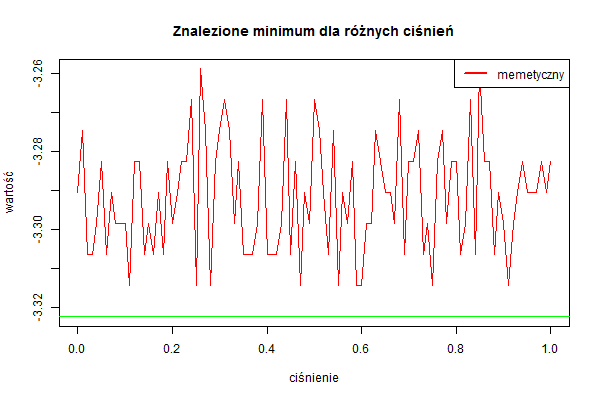
\includegraphics[width=0.95\textwidth]{./assets/Hartman6pressel.png}
	\caption{Jakość rozwiązań dla różnych wartości ciśnienia algorytmu hybrydowego}
	\label{fig:hybridpressel}
\end{figure}

\fbi
Wartości na wykresie (rys.~\ref{fig:hybridpressel}) różnią się od siebie o nie więcej niż 0,06. Oznacza to niski wpływ ciśnienia na rezultat algorytmu. Nie zauważalne są trendy wartości wraz ze wzrostem ciśnienia.


\begin{figure}[H]
	\centering
	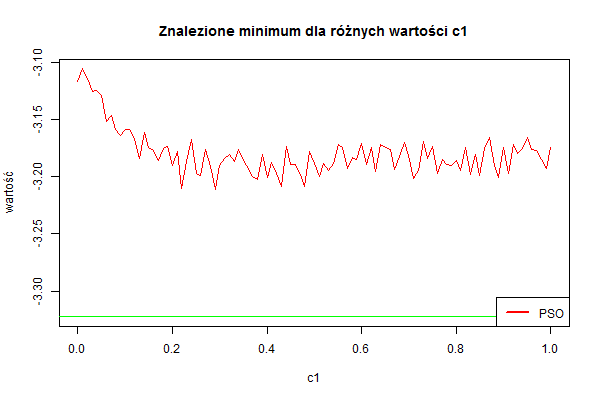
\includegraphics[width=0.95\textwidth]{./assets/Hartman6c1.png}
	\caption{Jakość rozwiązań dla różnych wartości c1 algorytmu PSO}
	\label{fig:psoc1}
\end{figure}

\fbi
Z przeprowadzonych badań najlepsze rezultaty otrzymano dla wartości c1 przekraczających 0,2. Po jej różnice spowodowane są heurystyką algorytmu, a nie parametrem.


\begin{figure}[H]
	\centering
	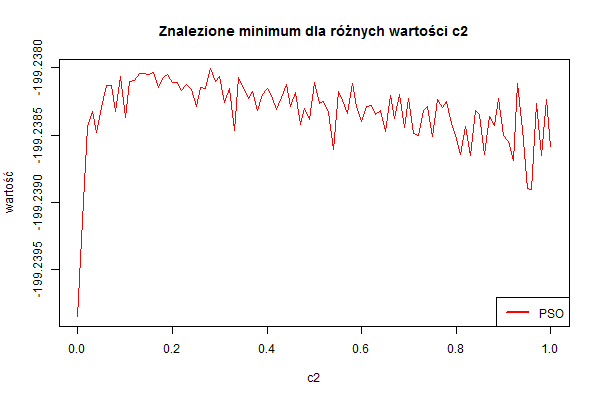
\includegraphics[width=0.95\textwidth]{./assets/Hartman6c2.png}
	\caption{Jakość rozwiązań dla różnych wartości c2 algorytmu PSO}
	\label{fig:psoc2}
\end{figure}

\fbi
Tak jak w przypadku parametru c1 najlepsze rezultaty uzyskano po przekroczeniu wartości 0,2. Jednak w tym wypadku można zauważyć powolne pogorszanie się wyników im większy parametr c2. 

\newpage
\section{Podsumowanie}
\paragraph{}
W trakcie prowadzonych badań przetestowano algorytmy w wariantach genetyczny prosty, genetyczny prosty z własną funkcją mutacji, hybrydowy prosty wraz z własną funkcją, TSP oraz PSO.

\fbi
Zmiana funkcji mutacji nie spowodowała znaczących zmian w jakości otrzymywanych rozwiązań. Jej działanie jest porównywalne z zaimplementowaną funkcją.

\fbi
Własna funkcja mutacji dla problemu TSP pogorszyła rezultaty o ok. 10 punktów procentowych.



\newpage
\begin{thebibliography}{40}

\bibitem{test1}
Artur Suchwałko ,,Wprowadzenie do R dla programistów innych języków'' https://cran.r-project.org/doc/contrib/R-dla-programistow-innych-jezykow.pdf

\bibitem{test2}
Luca Scrucca ,,Package GA''
https://cran.r-project.org/web/packages/GA/GA.pdf

\bibitem{test3}
Surjanovic, S. \& Bingham, D. (2013). ,,Virtual Library of Simulation Experiments: Test Functions and Datasets.'' Retrieved April 3, 2017, from http://www.sfu.ca/~ssurjano.

\bibitem{test4}
Momin Jamil, Xin-She Yang ,,A literature survey of benchmark functions for global optimization problems'', Int. Journal of Mathematical Modelling and Numerical Optimisation, Vol. 4, No. 2, pp. 150–194. (2013)

\bibitem{test5}
Ajith Abraham, Aboul-Ella Hassanien, Patrick Siarry, Andries Engelbrecht, ,,Foundations of Computational Intelligence Volume 3'' (2009)

\bibitem{test6}
Onay Urfalioglu, Orhan Arikan ,,Self-adaptive randomized and rank-based differential evolution for multimodal problems'' (2011)

\end{thebibliography}

\end{document}